\chapter{Módulo BD}
\noindent
Este capítulo tem o objetivo de abordar o último módulo desenvolvido para atender o objetivo proposto: o módulo do BD. Ele é responsável por oferecer o armazenamento persistente ao sistema e sua edição, possibilitando a visualização das faltas e sua alteração. As atividades de consulta e alteração da papeleta são realizadas através de um servidor web, desenvolvido nesse último módulo. Ele está relacionado aos requisitos funcionais \textit{RF02 - Verificar lista de presença} e   \textit{RF03 - Editar lista de presença}. Sobre o banco de dados a ser empregado, o \textit{RN02 - O banco de dados, no qual se fará o armazenamento persistente, deve ser PostgreSQL} torna isso claro. Além disso, o módulo encontra-se relacionado com os 3 casos de uso \textit{UC-01 Apurar falta, UC-02 Editar Lista de presença, UC-03 Verificar Lista de Presença}.

\section{Conceito Geral do módulo}
\noindent
Segundo \citep{bd}, os bancos de dados e suas tecnologias representam um papel crítico nos mais diversos sistemas nos quais se inserem, sendo que o nome banco de dados está relacionado a um conjunto de dados relacionados. No sistema proposto, esse conjunto de dados seria a composição das informações relacionadas à presença dos alunos, ou seja, disciplina, tempo de aula, matrícula do aluno, entre outros.

O banco de dados escolhido foi o \textit{PostgreSQL}, visando atender ao RN02 que estabelece que "o banco de dados, no qual se fará o armazenamento persistente, deve ser PostgreSQL". Segundo \citep{postsql}, o \textit{PostgreSQL} é um banco de dados relacional, com código aberto e que usa e estende a tradicional linguagem SQL. Ele teve origem na Universidade da Califórnia em Berkeley, no ano de 1986. Nesse contexto, o banco de dados relacional conta com mais de 30 anos de desenvolvimento e aperfeiçoamento. A versão escolhida foi a 9.6.10. Optou-se por utilizar o \textit{pgAdmin III}, em sua versão 1.22.2. O \textit{pgAdmin III}, segundo \citep{pgadmin}, é uma ferramenta para o gerenciamento de banco de dados \textit{PostgreSQL} que possui interface gráfica e ferramentas que auxiliam no gerenciamento e manutenção do banco. Sobre a licença, \citep{pgadmin} informa que a ferramenta é disponibilizada gratuitamente. 


\section{Modelagem do Banco de Dados}
\noindent 
O Modelo Entidade-Relacionamento, segundo \citep{bd}, é um modelo conceitual, muito popular, que trabalha com uma abstração de alto nível, empregando entidades, relacionamentos e atributos em sua modelagem.\citep{bd} explica ainda que o Diagrama Entidade-Relacionamento (ER) é a representação gráfica para um esquema. Buscou-se modelar um banco de dados de maneira simplificada, mas que atenda ao propósito do sistema de registrar a apuração das faltas por tempo de aula. Para a construção do Diagrama ER, utilizou-se o software brModelo 3.0. \citep{brmodelo} informa que ele foi desenvolvido por Carlos Henrique Cândido, e trata-se de uma ferramenta para a modelagem relacional. Destaca-se o fato do software desenvolvido por Carlos Cândido ser nacional e gratuito.    

A figura \ref{fig:figura60aa} ilustra o Diagrama ER para o sistema. Nele, tem-se as entidades \textit{aluno, turma, disciplina, professor, aula}. Cada aluno está matriculado em uma turma e cada turma cursa uma disciplina. Cabe aqui observar que, no Instituto Militar de Engenharia, os alunos devem cursar, obrigatoriamente, as disciplinas previstas para aquele semestre. Assim sendo, uma turma tem sua grade  de disciplinas rígida, tendo sido determinadas previamente as disciplinas a serem cursadas em um dado semestre. Um ou mais professores podem ministrar uma disciplina ao longo do semestre. Ao evento específico no qual um professor ministra uma disciplina, durante um intervalo predefinido de tempo, deu-se o nome de aula. Optou-se por considerar aula como sendo uma entidade devido à ênfase do sistema. Por fim, o aluno pode comparecer a uma aula ou não. Pode-se notar que aluno e professor guardam certa semelhança, sendo possível para ambos herdarem da entidade pessoa, o que não foi feito no diagrama apenas com a finalidade de torná-lo mais legível. Quanto a cardinalidade do relacionamento, optou-se por seguir a terminologia proposta por \citep{bdcardinalidade}, por exemplo, um aluno está matriculado em uma única turma, podendo uma turma ter um ou mais alunos. 

\begin{figure}[!ht]
	\centering
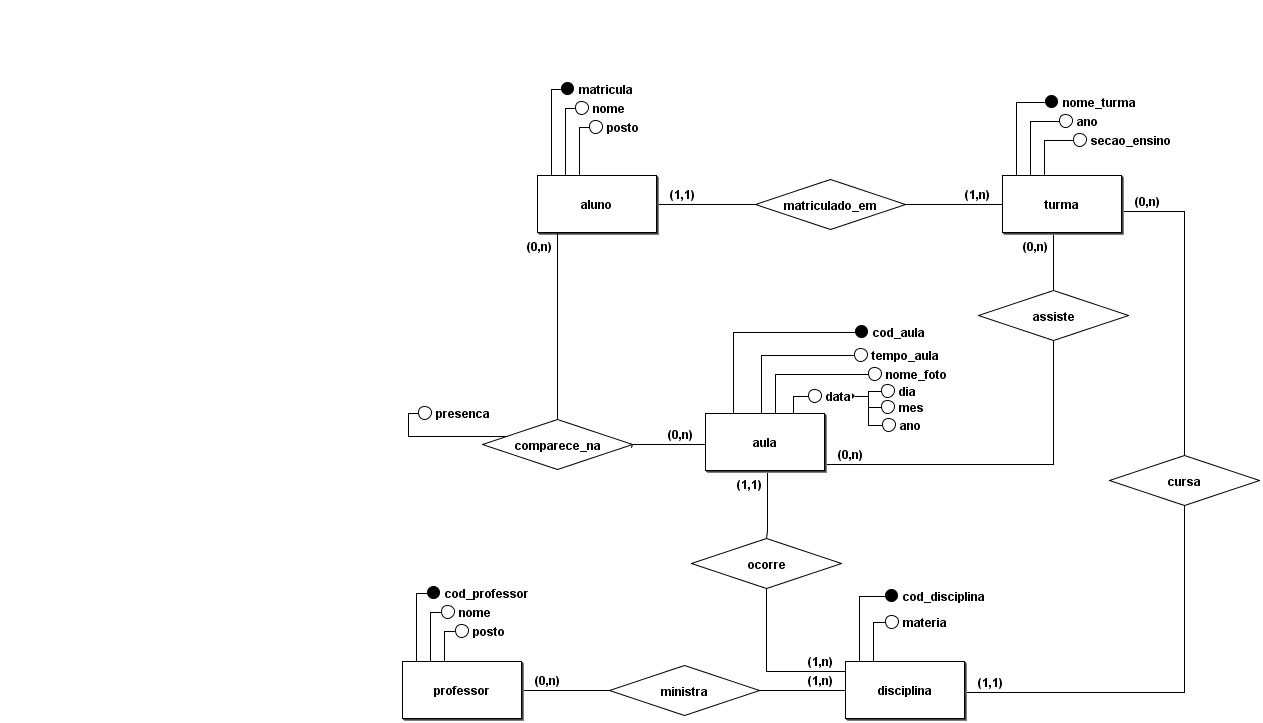
\includegraphics[width=1\textwidth]{img/Conceitual_1.png}   
	\caption{Diagrama ER do sistema}
	\label{fig:figura60aa}
\end{figure}


Na fase seguinte, usando o modelo ER, construiu-se o modelo de dados relacional. \citep{bd} explica que esse modelo trata o banco de dados como sendo um conjunto de relações. Representou-se através da figura  \ref{fig:figura60ab} o Diagrama para o esquema do banco de dados relacional tchau\_papeleta.  Quanto ao formato da representação, adotou-se o que \citep{bd} sugere em seu capítulo 5, página 98.  

\begin{figure}[!ht]
	\centering
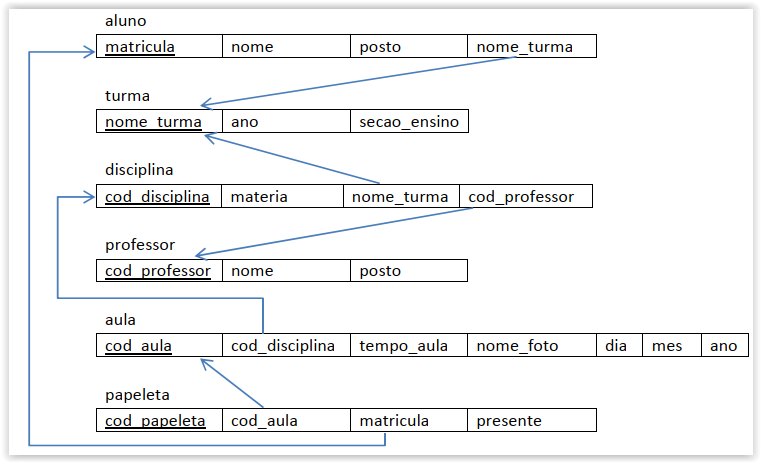
\includegraphics[width=1\textwidth]{img/relacional.PNG}   
	\caption{Diagrama para o esquema do banco de dados relacional tchau\_papeleta}
	\label{fig:figura60ab}
\end{figure}

\section{Criação do esquema}
Na fase seguinte, criou-se um banco de dados relacional do tipo postgreSQL. No banco de dados proposto, a tabela \textbf{aluno} tem as colunas matrícula, nome, posto e cod\_turma. A matrícula, por ser um identificador único, é a chave primária. Para a coluna posto, os alunos militares têm a abreviação de sua graduação ou posto. Os alunos da reserva receberiam a palavra \textit{civil}. O nome\_turma faz referência à turma, sendo uma chave estrangeira. A \textbf{turma} seria composta pelo nome\_turma, um identificador único da turma que funciona como chave primária, além do ano e da secao\_ensino. O ano se refere ao ano da graduação na qual a turma se encontra e.g: o 5º ano teria ano igual a 5. A secao\_ensino representa a seção de ensino, sendo essa uma sigla sigla, e.g: SE8. O \textbf{professor} é composto por um cod\_professor, chave primária, além do nome e posto. A \textbf{disciplina} é formada por cod\_disciplina, matéria (nome por extenso da disciplina), nome\_turma (chave estrangeira fazendo referência à turma), cod\_professor1 e cod\_professor2 (chaves estrangeiras que referenciam  professor). Nesse momento, vale destacar que preferiu-se utilizar 2 campos para professor, priorizando o desempenho ao espaço, isso se explica pois no IME, as disciplinas tem, em geral, no máximo 2 professores encarregados de uma disciplina. Criar uma tabela relacionando professor e disciplina, nesse caso teria um impacto negativo no desempenho, e traria um benefício de evitar redundância pequeno. A \textbf{aula} é composta por cod\_aula (chave primária), dia, mês e ano (compondo a data), cod\_disciplina (chave estrangeira que se refere à disciplina), tempo\_aula e nome\_foto. Por fim, a \textbf{papeleta} é composta por cod\_papeleta (chave primária), cod\_aula (chave estrangeira que refere aula), matrícula (chave estrangeira que refere aluno). Além desses, ter-se-á a coluna presente, um \textit{boolean} no qual  \textit{true} representa que o aluno compareceu à aula e  \textit{false} que o aluno faltou.

Criou-se um \textit{Database} denominado IME. A partir dele, criou-se o esquema e suas tabelas. A figura \ref{fig:figura60a} mostra a criação do esquema denominado \textit{tchau\_papeleta}. A seguir, as tabelas \textit{turma, aluno, professor, disciplina, aula e papeleta} são criadas. Após a criação do esquema e tabelas, fez-se a inserção de dados, conforme ilustrado na figura \ref{fig:figura61a}. Para o funcionamento do sistema, os professores, alunos, disciplinas e turmas já devem ter sido previamente cadastrados, conforme ilustra a figura \ref{fig:figura61a}.  

\begin{figure}[!ht]
	\centering
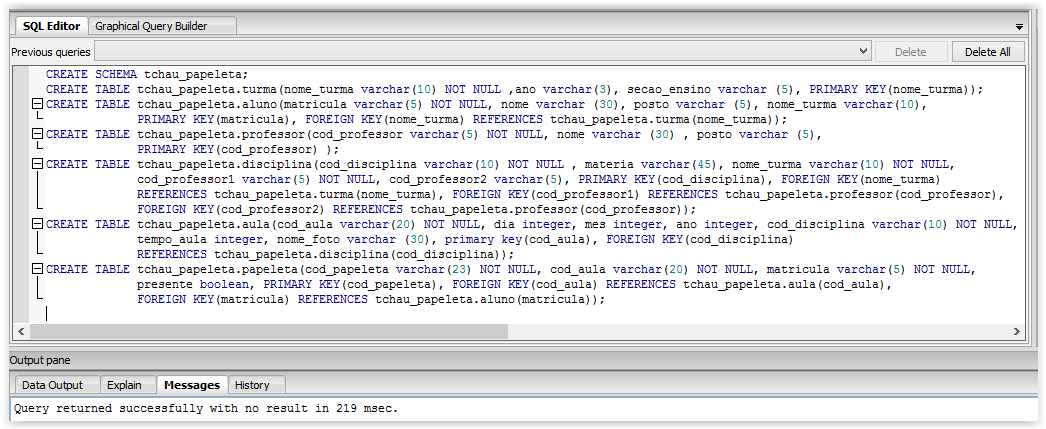
\includegraphics[width=1\textwidth]{scriptcriacao.PNG}   
	\caption{Criação usando o pgAdmin III}
	\label{fig:figura60a}
\end{figure}

\begin{figure}[!ht]
	\centering
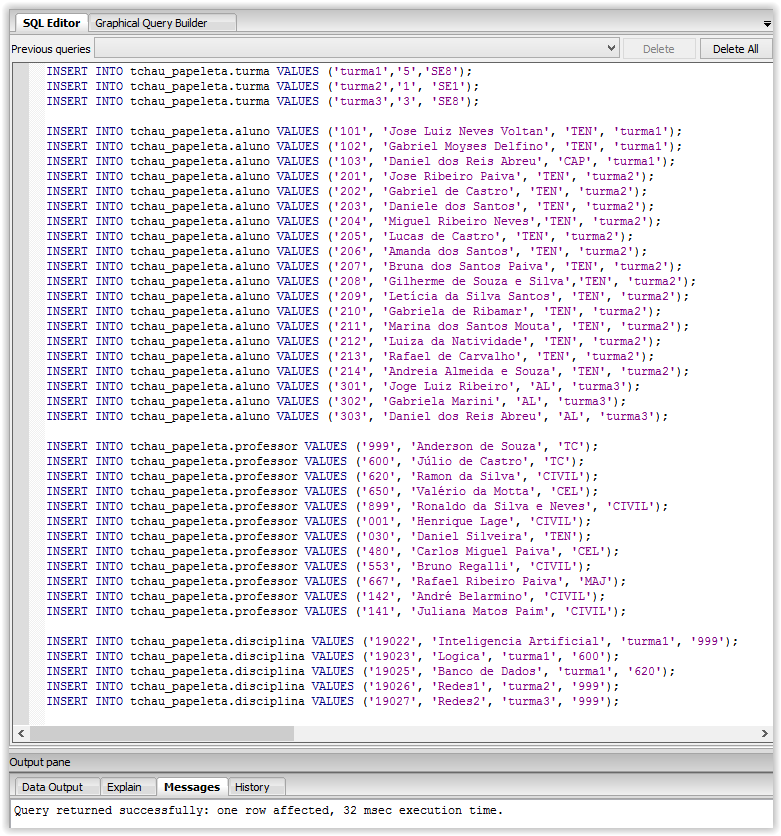
\includegraphics[width=1\textwidth]{populacao.PNG}   
	\caption{Inserção dos dados no esquema \textit{tchau\_papeleta}}
	\label{fig:figura61a}
\end{figure}

Quando o professor, utilizando o aplicativo "Tchau Papeletas", fizer o envio da fotografia da turma, ele também enviará nome da turma, representado no esquema como \textit{nome\_turma}, e o nome da disciplina, que aparecerá como \textit{materia}. Essas duas informações serão necessárias para identificar a turma de maneira inequívoca, uma vez que  uma mesma matéria pode ser oferecida para mais de uma turma. Por exemplo, a matéria "Fenômenos de Transporte" é ministrada com o mesmo nome tanto para o 3º ano de Engenharia Química quanto para o 3º ano de Engenharia da computação. Trata-se, contudo, de disciplinas distintas, com códigos (\textit{cod\_disciplina}) e conteúdo diferentes. A figura \ref{fig:figura62a} exibe a consulta para, a partir dessas duas informações, encontrar-se o \textit{cod\_disciplina}. No exemplo, \textit{nome\_turma} = 'turma1' e \textit{materia} = 'Logica', retornando como resultado o \textit{cod\_disciplina} = 19023.

\begin{figure}[!ht]
	\centering
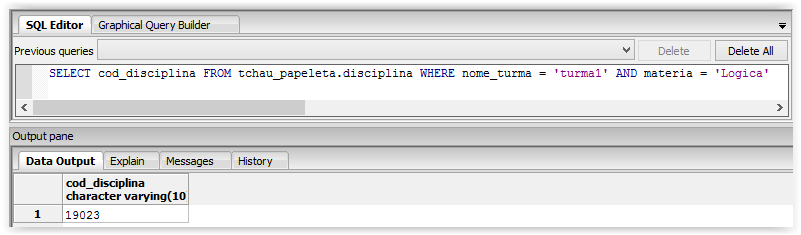
\includegraphics[width=1\textwidth]{consulta1.PNG}   
	\caption{Consulta para obtenção da \textit{cod\_disciplina}}
	\label{fig:figura62a}
\end{figure}

Além desses, o professor também informará os tempo de aula, sendo a data composta por dia, mês e ano incluída pelo servidor. Com essas informações, ter-se-á parâmetros suficientes para criação da aula. A figura \ref{fig:figura63a} demonstra a inserção de uma aula ministrada no dia 05, mês 09 e ano 2018, referente à disciplina Lógica, ministrada para a turma1, (\textit{cod\_disciplina} = '19023'). Preencher-se-á o atributo \textit{nome\_foto} conforme apresentado no capítulo 4, referente ao módulo servidor. 

\begin{figure}[!ht]
	\centering
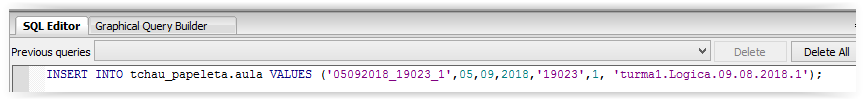
\includegraphics[width=1.0\textwidth]{consulta2.PNG}   
	\caption{Inserção de uma aula}
	\label{fig:figura63a}
\end{figure}

Após a inserção da aula, pode-se gerar para cada membro da turma a presença ou falta naquela aula. A figura \ref{fig:figura64a} mostra como obter a \textit{matrícula} dos alunos de uma turma. No exemplo, utiliza-se turma1. Por fim, a figura \ref{fig:figura65a} demonstra a inserção da presença ou falta de cada aluno dessa turma.  

\begin{figure}[!ht]
	\centering
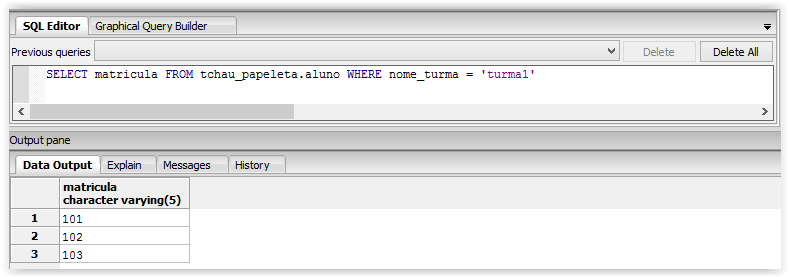
\includegraphics[width=1.0\textwidth]{consulta3.PNG}   
	\caption{Obtenção da relação de aluno (\textit{matrícula}) de uma turma}
	\label{fig:figura64a}
\end{figure}

\begin{figure}[!ht]
	\centering
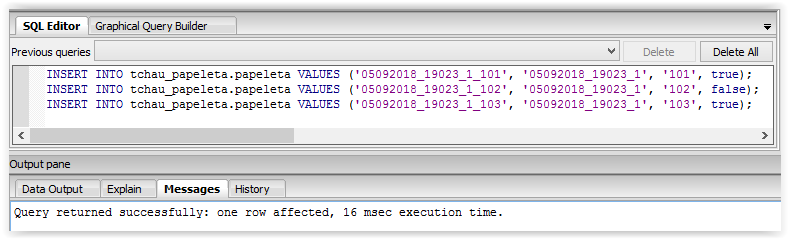
\includegraphics[width=1.0\textwidth]{consulta4.PNG}   
	\caption{Inserção da falta}
	\label{fig:figura65a}
\end{figure}


\section{Conexão com o Banco de Dados através do Python DB API}
Depois que a fotografia é enviada para o servidor e  as faces são reconhecidas, registrar-se-á essas informações no banco de dados. Para a integração entre o código escrito em Python e o PostgreSQL, fez-se uso do \textit{Psycopg}. Segundo \citep{Psycopg}, o \textit{Psycopg} é o adaptador mais popular para essa finalidade. O \textit{"Python DB API 2.0"} possui licença gratuita e segue a política \textit{GNU Lesser General Public License}. A versão escolhida foi a 2.7.5. 

Optou-se, então, por criar uma classe denominada Conecta (arquivo conexao.py), que apresenta os métodos necessários para a manipulação dos dados. Em seu construtor, realizar-se-á a conexão com o banco de dados, usando como parâmetros \textit{host, database, usuário} e \textit{senha}. A classe possui ainda, dentre outos, os métodos genéricos para consulta e inserção (cláusulas \textit{select} e \textit{insert}). 

Quando uma fotografia de uma turma é recebida, o primeiro passo é identificar se aquela fotografia é a primeira ou não. Caso seja a primeira, deve-se criar a linha aula correspondente àquela fotografia e suas informações, além da papeleta de cada aluno com o atributo presente recebendo \textit{false}. Caso não seja a primeira isso não deve ser feito sob pena de apagar a presença de um aluno apurada anteriormente. Para essa verificação, optou-se por, dentro do método \textit{inserir\_aula}, consultar se, de fato, aquela inserção é necessária ou não. Caso necessário, além da inserção, cria-se a papeleta de cada aluno como mencionado. O retorno do referido método é o \textit{cod\_aula}.  O passo seguinte é criar um método nessa classe tal que, recebendo a matrícula do aluno que teve sua face detectada, seja permitido alterar, na linha correspondente da tabela papeleta, o atributo presente de \textit{false} para \textit{true}. 

\section{Acesso ao Banco de Dados para Consulta e Atualização}
Para o atendimento dos requisitos RF02 e RF03, definidos no capítulo de modelagem do sistema, foi implementado um serviço \textit{web}, no qual o cliente consiste em um formulário HTML e o servidor em uma página JSP. No formulário, constam os seguintes campos de preenchimento: dia, mês, ano, tempo de aula, turma e disciplina . Com essa informação é possível fazer uma consulta que retorna a matrícula, o posto e o nome de todos os alunos da turma, bem como a situação de cada um quanto a frequência ao tempo de aula especificado. 
A estrutura desse serviço \textit{web} caracteriza-se por uma página inicial, ilustrada na figura \ref{fig:figura66}, que exibe dois \textit{links} de acesso: 
\textit{Link} de acesso para a atualização, que permite a consulta e atualização do banco de dados, isso é, os dados são exibidos na forma de uma tabela e o usuário pode alterar a presença ou falta do aluno; e
\textit{Link} que permite apenas consulta, voltado para alunos e coordenadores.
Ambos os \textit{links} direcionam o usuário para a página que contém o formulário, figura \ref{fig:figura67}, o qual, ao ser enviado, direciona para a página JSP, que se encarrega de fazer a manipulação do banco de dados, conforme mostra a figura \ref{fig:figura68}. Caso o formulário seja enviado pelo professor, o servidor exibe uma tabela com o resultado da consulta e contendo uma coluna com botões cuja função é modificar a situação do aluno, de presente para ausente ou o inverso. Se for aluno ou coordenador, o servidor retorna retorna a mesma tabela do caso anterior, porém sem as permissões de alteração e exibição dos botões. 
\begin{figure}[!ht]
	\centering
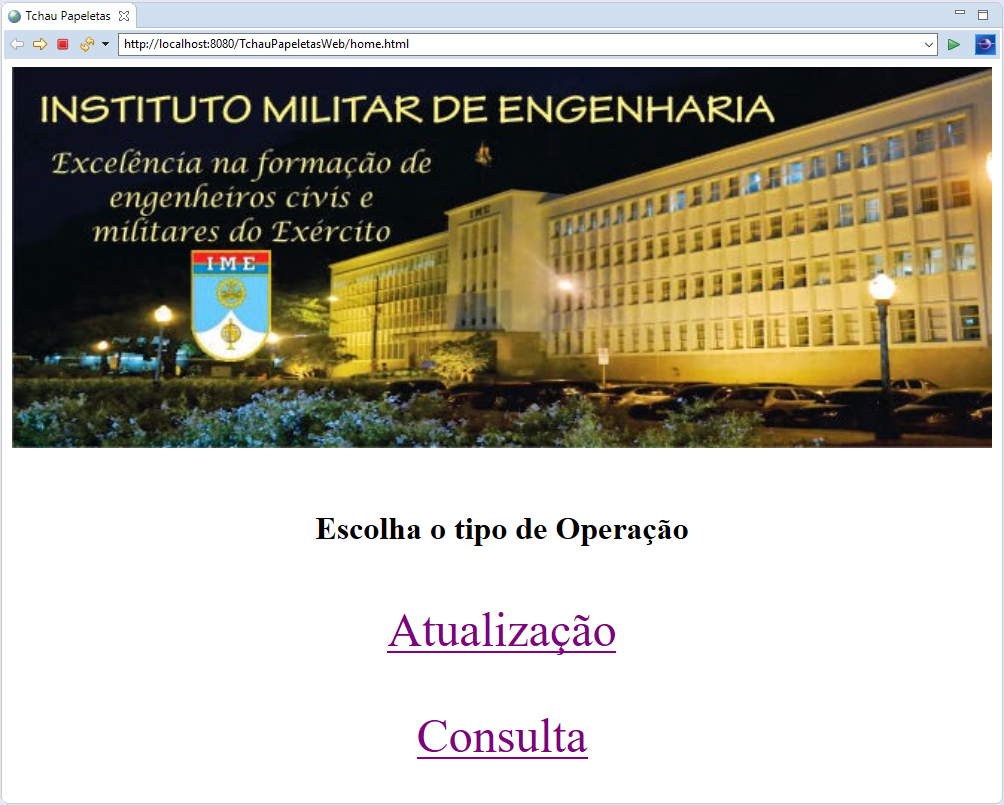
\includegraphics[width=0.70\textwidth]{img/home_page.png}  
	\caption{Página inicial do serviço(\textit{web})}
	\label{fig:figura66}
\end{figure}

\begin{figure}[!ht]
	\centering
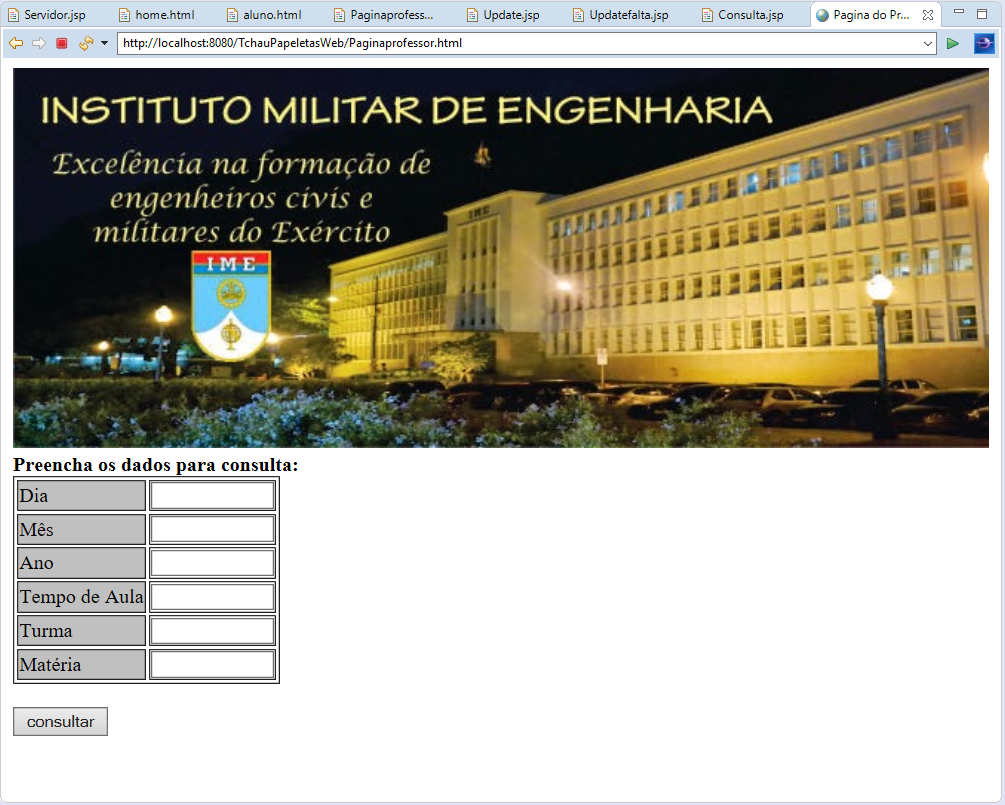
\includegraphics[width=0.70\textwidth]{img/pagina_de_consulta.png}   
	\caption{Página de preenchimento e envio de formulário html}
	\label{fig:figura67}
\end{figure}

\begin{figure}[!ht]
	\centering
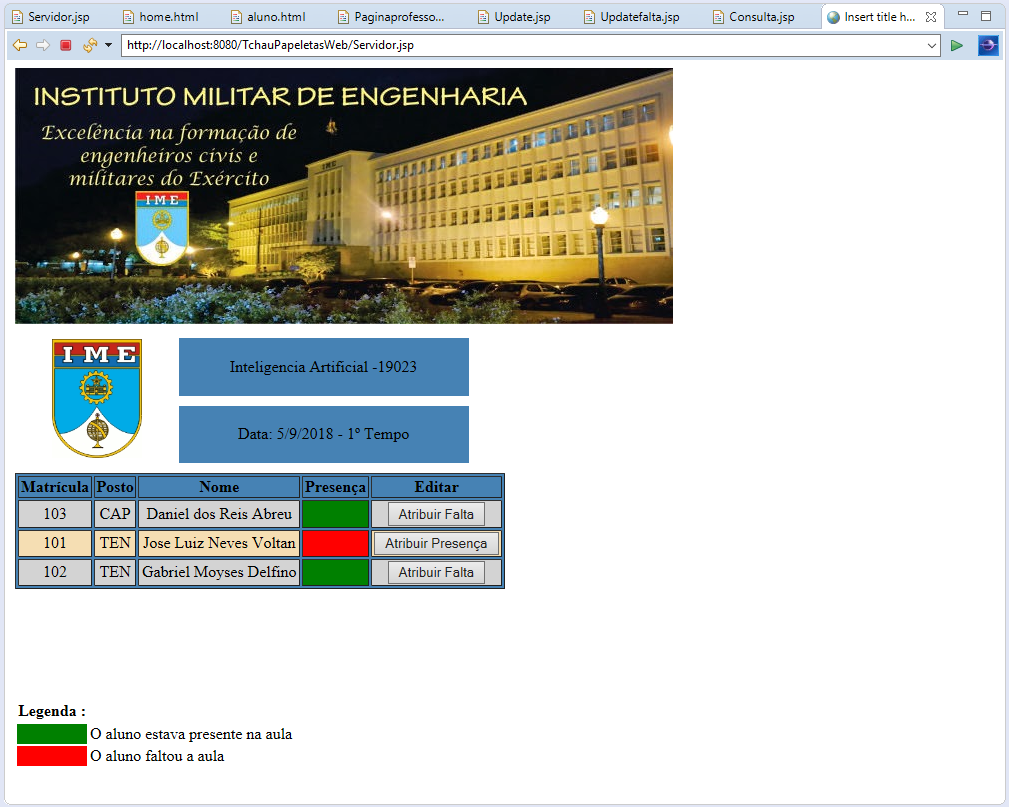
\includegraphics[width=0.70\textwidth]{img/servidorjsp.png}   
	\caption{Página de exibição do resultado da operação Atualização}
	\label{fig:figura68}
\end{figure}


Conforme mencionado anteriormente, a transação de atualização é feita pelos botões. Cada botão, ao ser pressionado, atualiza a frequência da linha a qual se refere. Quando a operação é bem sucedida, o usuário é notificado do sucesso por uma mensagem de texto, exibida abaixo da tabela, e também pela mudança de cor do campo presença e do próprio botão acionado. É importante mencionar que durante essas atualizações e notificações a página não precisa ser recarregada, evitando-se, assim, a necessidade de uma nova consulta para obter a tabela a cada atualização feita. Isso é possível por meio de requisições HTTP assíncronas, conhecidas como AJAX, que permitem a troca de dados entre cliente e servidor em segundo plano e a atualização de partes da página sem a necessidade de recarregar a página como um todo, \citep{W3}. A figura \ref{fig:figura69} mostra um exemplo de notificação. 

\begin{figure}[!ht]
	\centering
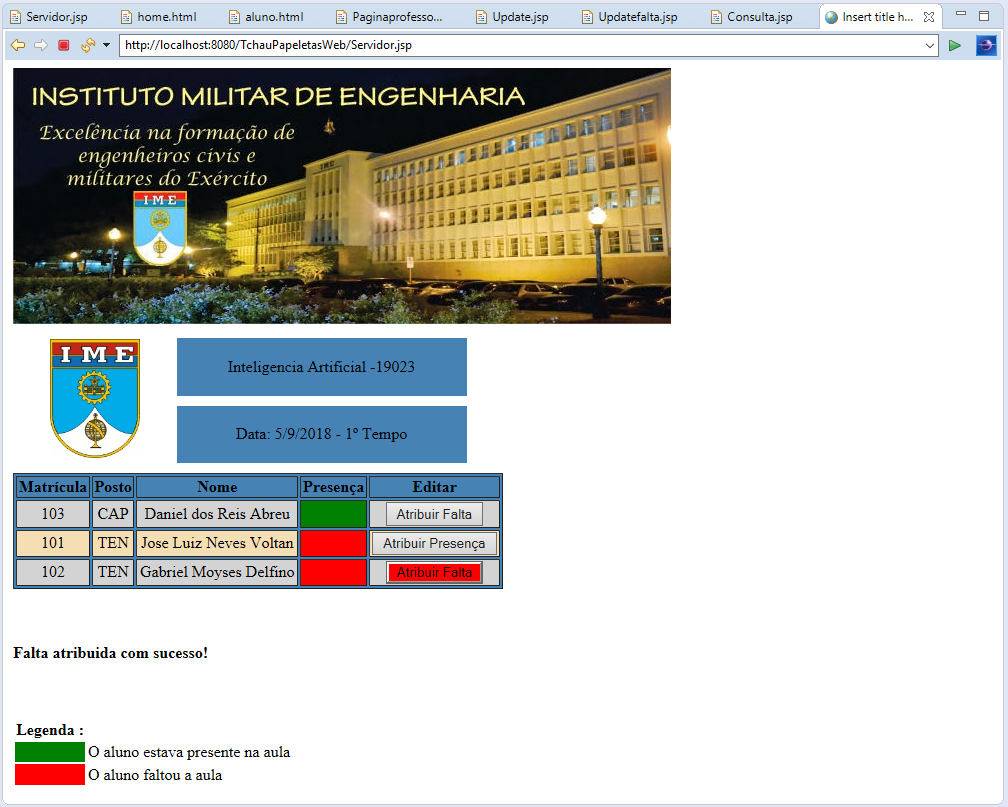
\includegraphics[width=0.70\textwidth]{img/atualizacao.png}   
	\caption{Exemplo de atualização}
	\label{fig:figura69}
\end{figure}

Perceba que devido à questões temporais limitantes do projeto, não se projetou um sistema de autenticação de usuário. Como oportunidade de melhoria, pode se ter um cadastro com login e senha dos usuários, que permita a separação das operações conforme a função do usuário, assim um aluno não poderia atualizar a lista de presença de uma turma, mas um professor sim. Além disso, poderia se dar um tratamento especial aos campos, evitando tentativas de injeção SQL. 






